% !TEX root = ../thesis.tex

\section{Event Selection and Categorization}
\label{sec:events}

% Goal of event selection
In subsection~\ref{subsec:expEvent}, we described the expected event topology for the \WV/\WH dibosonic resonance that this work searches for.
In particular, the semileptonic decay produces a highly energetic lepton ($e$ or $\mu$) and large \Etmiss from the neutrino from the \Wtolnu decay, a large-radius jet from the hadronic \Vtoqqbarpr or \Htobbbar decay, and forward-facing \VBF jets for \VBF-produced resonances.
To select for possible events that exhibit the expected final state structure, selection cuts must be made that capture the expected behavior and reduce background.
This section provides an overview of the cuts that were made in the analysis to optimize the search for the \WV/\WH dibosonic resonance.

\subsection{Trigger}

% Trigger paths
There are multiple HLT trigger paths that used for recording the data that this analysis uses.
Most of the data are collected from the single electron and single muon triggers, with the remainder coming from the single photon, EGamma, and MET triggers.
For each year we use different paths, which are listed in tables~\ref{tab:triggers2016}, \ref{tab:triggers2017}, and \ref{tab:triggers2018} for the years Run 2, respectively.

\begin{table}[htbp]
  \centering
  % !TEX root = ../../thesis.tex
\footnotesize
\begin{tabular}{l|l|c}
  \hline
  Dataset        & HLT paths                                    & Description\\
  \hline \hline
  \ttfamily SingleElectron/& \ttfamily HLT\_Ele27\_WPTight\_Gsf\_v*                 & $\pt>27\unit{GeV}$, Tight WP for ele ID  \\
  \ttfamily SinglePhoton   & \ttfamily OR HLT\_Ele45\_WPLoose\_Gsf\_v*              & $\pt>45\unit{GeV}$, Loose WP for ele ID  \\
                 & \ttfamily OR HLT\_Ele115\_CaloIdVT\_GsfTrkIdT\_v*      & $\pt>115\unit{GeV}$  \\
                 & \ttfamily OR HLT\_Photon175\_v*                        & $\Et>175\unit{GeV}$  \\
  \hline
  \ttfamily SingleMuon     & \ttfamily HLT\_Mu50\_v*                                & $\pt>50\unit{GeV}$ \\
                 & \ttfamily OR HLT\_TkMu50\_v*                           & tracker muon, $\pt>50\unit{GeV}$ \\
  \hline
  \ttfamily MET            & \ttfamily HLT\_PFMETNoMu120\_PFMHTNoMu120\_IDTight\_v* & $\Etmiss>120\unit{GeV}$ \\
  \hline
\end{tabular}

  \caption{
    HLT paths used in 2016 data and MC.
  }
  \label{tab:triggers2016}
\end{table}

\begin{table}[htbp]
  \centering
  % !TEX root = ../../thesis.tex
\footnotesize
\begin{tabular}{l|l|c}
  \hline
  Dataset        & HLT paths                                    & Description\\
  \hline \hline
  \ttfamily SingleElectron/& \ttfamily HLT\_Ele32\_WPTight\_Gsf\_v*                 & $\pt>32\unit{GeV}$, Tight WP for ele ID  \\
  \ttfamily SinglePhoton   & \ttfamily OR HLT\_Ele35\_WPTight\_Gsf\_v*              & $\pt>35\unit{GeV}$, Tight WP for ele ID  \\
                 & \ttfamily OR HLT\_Ele115\_CaloIdVT\_GsfTrkIdT\_v*      & $\pt>115\unit{GeV}$  \\
                 & \ttfamily OR HLT\_Photon200\_v*                        & $\Et>200\unit{GeV}$  \\
  \hline
  \ttfamily SingleMuon     & \ttfamily HLT\_Mu50\_v*                                & $\pt>50\unit{GeV}$ \\
                 & \ttfamily OR HLT\_OldMu100\_v*                         & $\pt>100\unit{GeV}$ \\
                 & \ttfamily OR HLT\_TkMu100\_v*                          & tracker muon, $\pt>100\unit{GeV}$ \\
  \hline
  \ttfamily MET            & \ttfamily HLT\_PFMETNoMu120\_PFMHTNoMu120\_IDTight\_v* & $\Etmiss>120\unit{GeV}$ \\
  \hline
\end{tabular}

  \caption{
    HLT paths used in 2017 data and MC.
  }
  \label{tab:triggers2017}
\end{table}

\begin{table}[htbp]
  \centering
  % !TEX root = ../../thesis.tex
\scriptsize
\begin{tabular}{l|l|c}
  \hline
  Dataset        & HLT paths                                    & Description\\
  \hline \hline
  \ttfamily EGamma         & \ttfamily HLT\_Ele32\_WPTight\_Gsf\_v*                 & $\pt>32\unit{GeV}$, Tight WP for ele ID  \\
                 & \ttfamily OR HLT\_Ele115\_CaloIdVT\_GsfTrkIdT\_v*      & $\pt>115\unit{GeV}$  \\
  \hline
  \ttfamily SingleMuon     & \ttfamily HLT\_Mu50\_v*                                & $\pt>50\unit{GeV}$ \\
                 & \ttfamily OR HLT\_OldMu100\_v*                         & $\pt>100\unit{GeV}$ \\
                 & \ttfamily OR HLT\_TkMu100\_v*                          & tracker muon, $\pt>100\unit{GeV}$ \\
  \hline
  \ttfamily MET            & \ttfamily HLT\_PFMETNoMu120\_PFMHTNoMu120\_IDTight\_v* & $\Etmiss>120\unit{GeV}$ \\
  \hline
\end{tabular}

  \caption{
    HLT paths used in 2018 data and MC.
  }
  \label{tab:triggers2018}
\end{table}

% Single electron thresholds
The single electron \pt thresholds used are 27, 45, and $115\unit{GeV}$ for 2016, 32, 25, and $115\unit{GeV}$ for 2017, and 25 and $115\unit{GeV}$ for 2018. % Check why the threshold is 25 and not 32 for 2018
Additionally, we apply an OR with \texttt{HLT\_Photon175} in 2016 with an \Et threshold of $175\unit{GeV}$, as well as with \texttt{HLT\_Photon200} in 2017 with $200\unit{GeV}$. % Need to find out what an OR is
These thresholds were applied as recommended by the CMS E/Gamma Physics Object Group (POG)~\cite{MuonPOG}.

% Single muon thresholds
For the muon thresholds, the main threshold is $50\unit{GeV}$ across all three years, with an OR for \texttt{HLT\_TkMu50} at $50\unit{GeV}$ in 2016, and an OR for \texttt{HLT\_OldMu100} in 2017 and \texttt{HLT\_TkMU100} in 2018 at $100\unit{GeV}$, as recommended by the Muon POG~\cite{MuonHLT2016,MuonHLT2017,MuonHLT2018}.

% Additional explanation of efficiencies?
% Possibly add subsection on prefiring weights

\subsection{Pileup Reweighting}

The data samples from all three Run 2 years have different pileup (PU) profiles than that of the simulation samples that were used for this analysis.
In order to account for this, we compute and apply PU weights to our samples and compare distributions for the number of primary vertices both with and without weights to the data.
Figure~\ref{fig:PUreweight} shows these distributions for Run 2.
The weights are computed using the recommended minimum bias cross section of $69.2\unit{mb}$. % Citation needed

\begin{figure}[htbp]
  \centering
  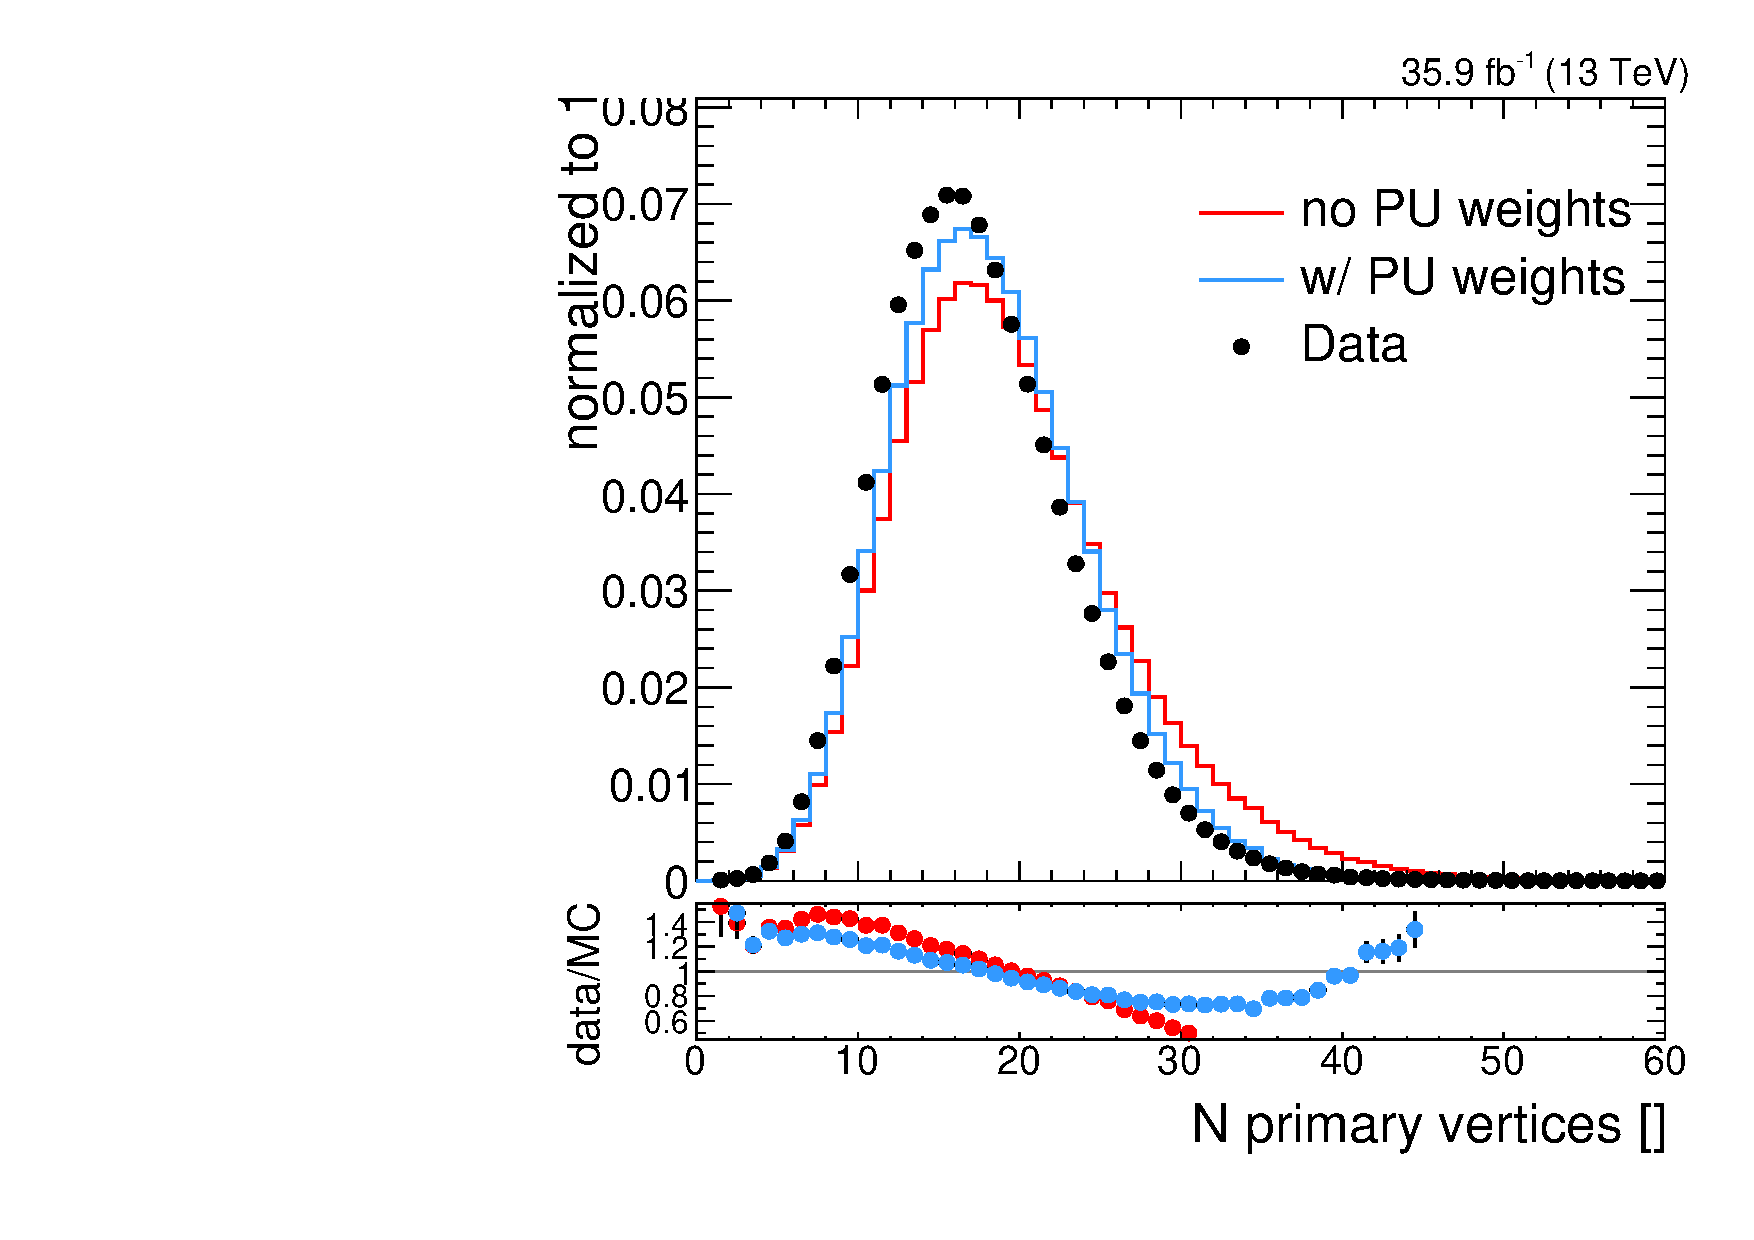
\includegraphics[width=0.45\textwidth]{fig/eventSelection/PUrewN_0_2016_nVert.pdf}
  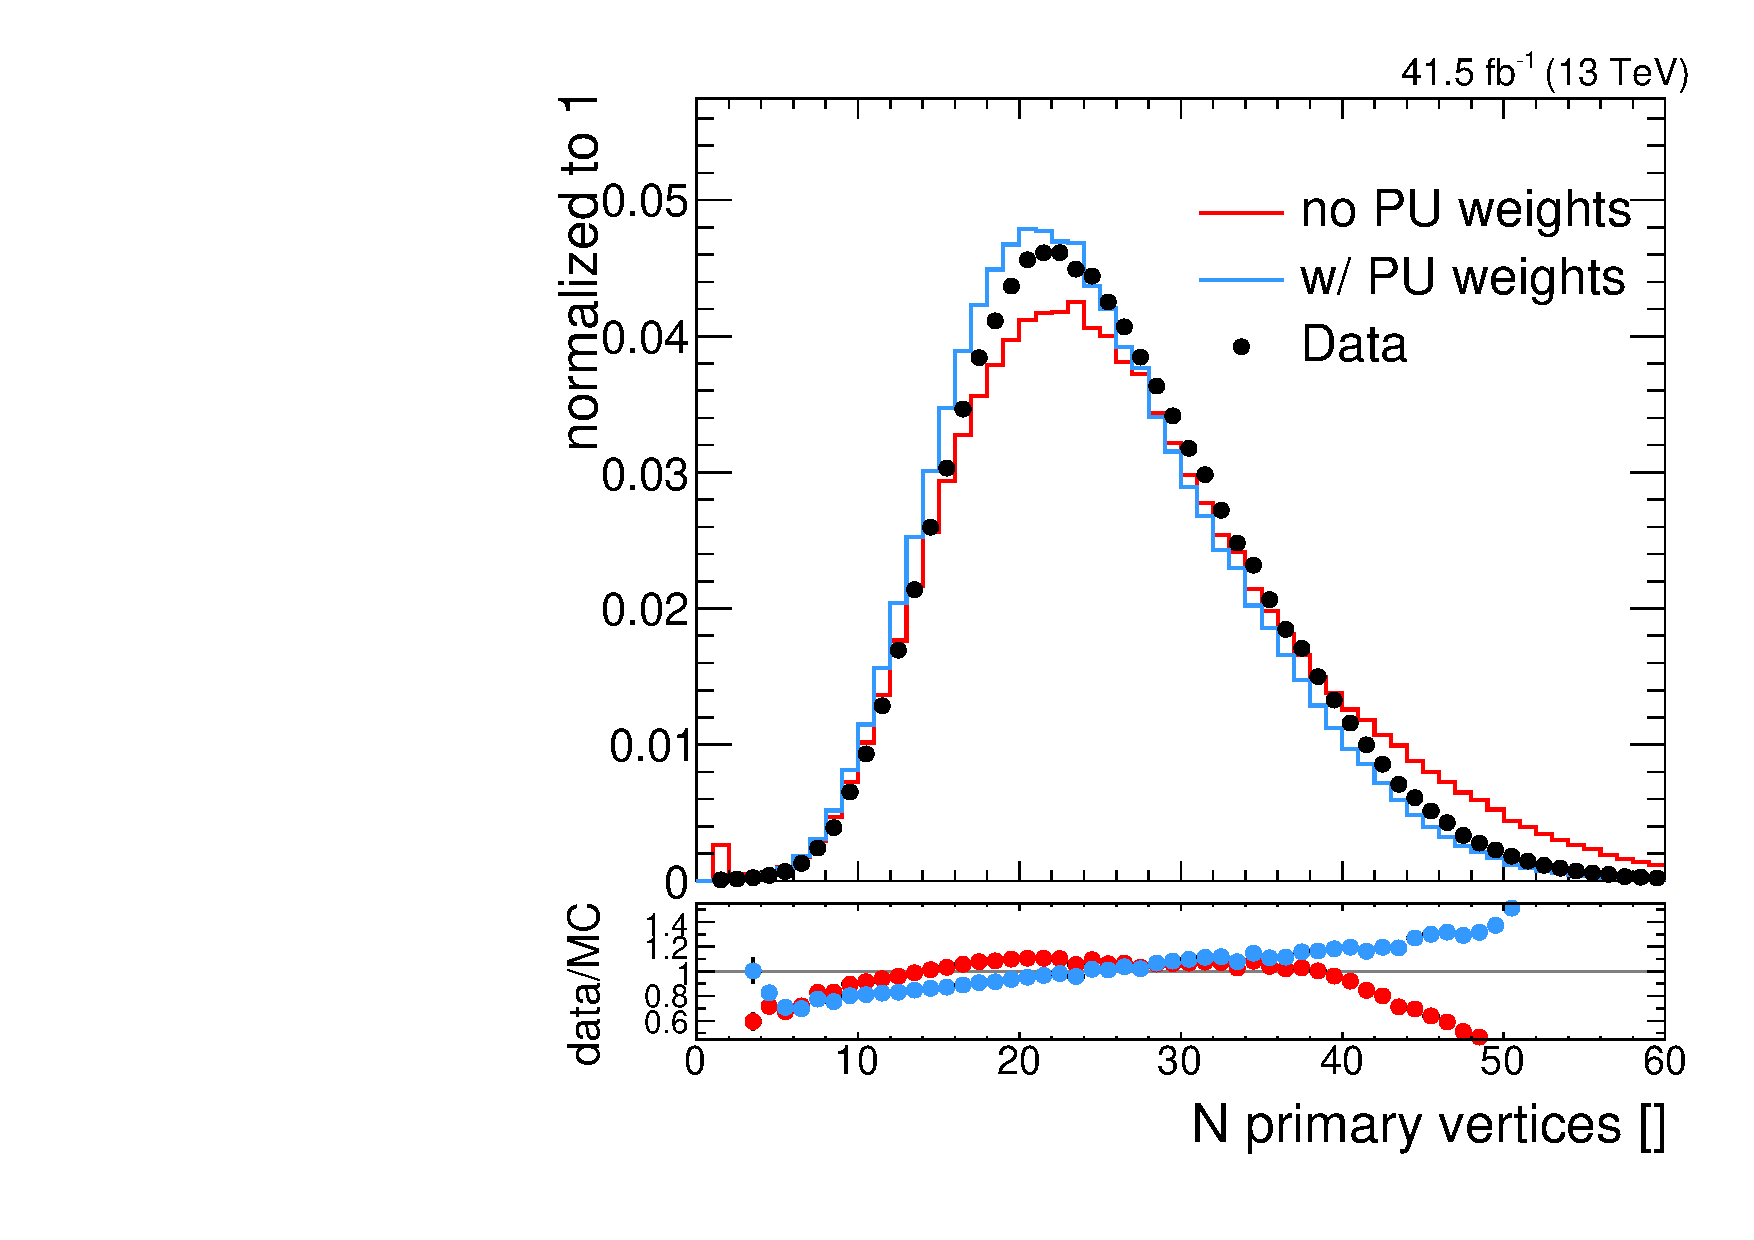
\includegraphics[width=0.45\textwidth]{fig/eventSelection/PUrewN_0_2017_nVert.pdf}\\
  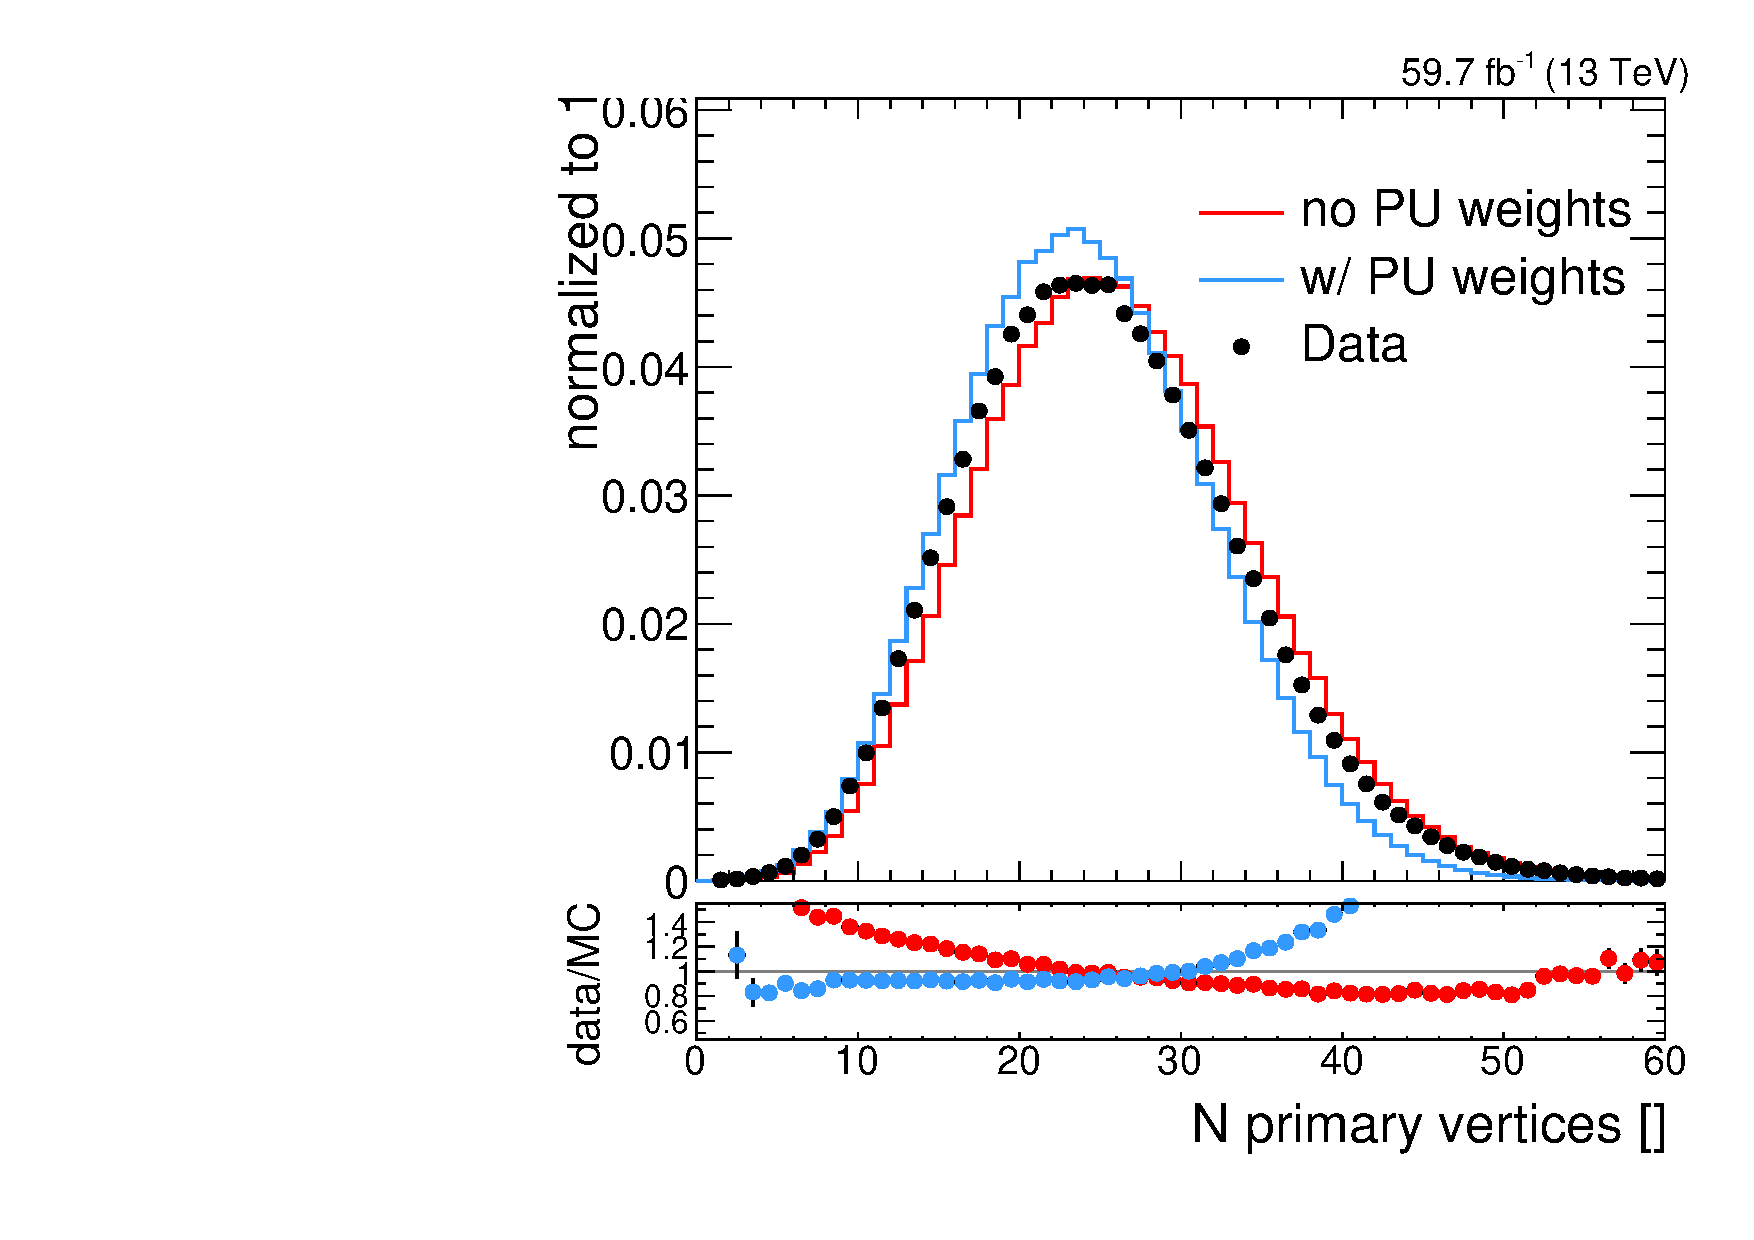
\includegraphics[width=0.45\textwidth]{fig/eventSelection/PUrewN_0_2018_nVert.pdf}
  \caption{
    Distribution of the number of primary vertices reconstructed in simulation before and after pileup reweighting, with data present, for 2016 (top left), 2017 (top right), and 2018 (bottom).
  }
  \label{fig:PUreweight}
\end{figure}

\subsection{Muon Selection}
\label{subsec:muonSelect}

% High-pT muon selection criteria
When selecting muons for the analysis, they must pass the following high-\pt muon identification criteria as provided by the CMS Muon POG~\cite{MuonSelection}:
\begin{itemize}
  \item The muon is reconstructed as a ``global'' muon.
  \item At least one muon-chamber hit included in the global-muon track fit or in the TuneP fit.
  \item Muon segments in at least two muon stations.
  \item The \pt relative error ($\sigma(\pt)/\pt$) of the muon best track is less than 30\%.
  \item Its tracker track has transverse impact parameter $d_{xy}<2\unit{mm}$ with respect to the primary vertex.
  \item The longitudinal distance of the tracker with respect to the primary vertex is $d_z<5\unit{mm}$.
  \item The muon track has at least one pixel hit.
  \item The muon track has at least six tracker layer hits.
\end{itemize}

% Further muon selection
In addition to the high-\pt muon identification criteria, for this analysis we also require each muon to have $\pt>55\unit{GeV}$ and to be confined to the region $|\eta|<2.4$.
We also apply an isolation requirement on the muons in order to further suppress background.
This is done using the full relative particle flow isolation using $\Delta\beta$ corrections, with the requirement that $I_\mathrm{rel}<0.05$.

Scale factors for muon ID as provided by the Muon POG are also applied~\cite{MuonPAGs}.
To appropriately apply these scale factors as they vary by year to the full Run 2 dataset, we weight them by the fraction of integrated luminosity for each year.
We also apply a scale factor for the isolation requirement, which is shown in figure~\ref{fig:muonIsoSF}.
This scale factor was derived on top of muon high-\pt ID, in boosted $Z$ and DY events over the full Run 2 period, which is found to be within 1\% from unity and smaller than the systematic uncertainty for the muon trigger/reco/ID of 5\% used in signal extraction.

\begin{figure}[htbp]
  \centering
  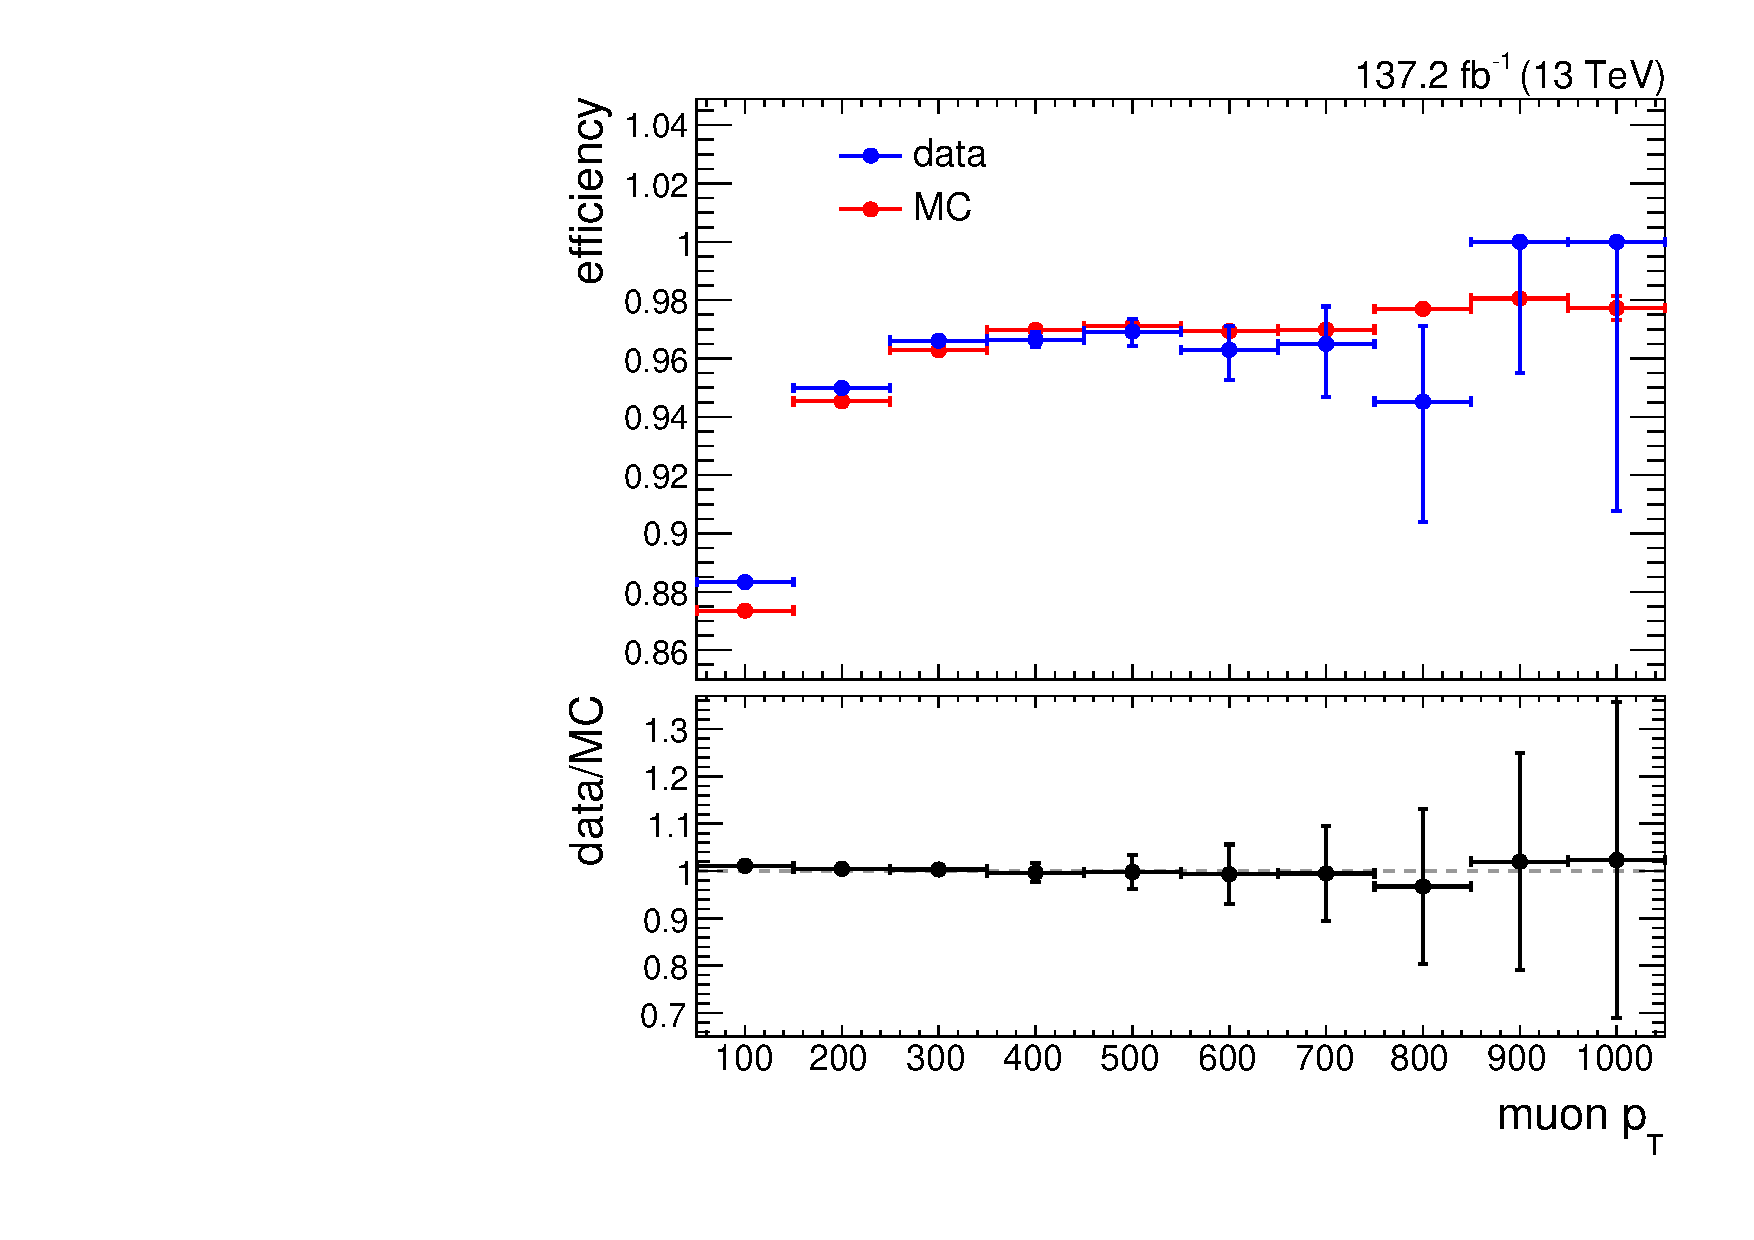
\includegraphics[width=0.65\textwidth]{fig/eventSelection/muonFullIsoSF.pdf}
  \caption{
    Efficiency in data and simulation and data/MC scale factor for muon isolation requirement.
  }
  \label{fig:muonIsoSF}
\end{figure}

\subsection{Electron Selection}
\label{subsec:elecSelect}

% Electron reconstruction
The electrons that are reconstructed from trigger primitives in the ECAL are required to pass the ``HEEP v7.0'' ID requirements as prescribed by the E/Gamma POG~\cite{HEEPV70}.
The ID requirements ensure that the reconstructed electrons from the ECAL energy deposits are paired with a high quality track from the inner tracker and have a shape consistent with an electromagnetic shower in the calorimeter.
These requirements are listed in table~\ref{tab:HEEPV70}.
For our analysis, we also require them to have $\pt>55\unit{GeV}$ and be within the pseudorapidity range $|\eta|<2.5$, except for the region $[1.4442,1.566]$. % Unsure why this range is excluded
We also apply scale factors for the HEEP ID requirements along with RECO scale factors as recommended by the E/Gamma POG~\cite{EgammaScale}.

\begin{table}[htbp]
  \centering
  % !TEX root = ../../thesis.tex
\footnotesize
\begin{tabular}{l|l|l}
  \hline
  Variable & Barrel & Endcap \\
  \hline
  \hline
  \multicolumn{3}{c}{Acceptance selections} \\
  \hline
  \Et & $\Et>35\unit{GeV}$ & $\Et>35\unit{GeV}$ \\
  $\eta$ & $|\eta_\mathrm{SC}|<1.4442$ & $1.566<|\eta_\mathrm{SC}|<2.5$ \\
  \hline
  \multicolumn{3}{c}{Identification selections}  \\
  \hline
  \texttt{isEcalDriven} & \texttt{true} & \texttt{true} \\
  $\Delta\eta_\mathrm{in}^\mathrm{seed}$ & $|\Delta\eta_\mathrm{in}^\mathrm{seed}|<0.004$ & $|\Delta\eta_\mathrm{in}^\mathrm{seed}|<0.006$ \\
  $\Delta\phi_\mathrm{in}$ & $|\Delta\phi_\mathrm{in}|<0.06$ & $|\Delta\phi_\mathrm{in}|<0.06$ \\
  $H/E$ & $H/E<1/E+0.05$ & $H/E<5/E+0.05$ \\
  $\sigma_{i\eta i\eta}$ & - & $\sigma_{i\eta i\eta}<0.03$ \\
  $\frac{E_{1\times5}}{E_{5\times5}}$, $\frac{E_{2\times5}}{E_{5\times5}}$ & $\frac{E_{1\times5}}{E_{5\times5}}>0.83$ or $\frac{E_{2\times5}}{E_{5\times5}}>0.94$ & - \\
  Inner lost layer hits & lost hits $\leq1$ & lost hits $\leq1$ \\
  Impact parameter, $d_{xy}$ & $|d_{xy}|<0.02$ & $|d_{xy}|<0.05$ \\
  \hline
  \multicolumn{3}{c}{Isolation selections}\\
  \hline
  EM + had depth 1 & $I<2+0.03\Et+0.28\rho$ & $I<2.5+0.28\rho$ ($\Et<50\unit{GeV}$) \\
  isolation, $I$ & & else $I<2.5+0.03(\Et-50\unit{GeV})+0.28\rho$ \\
  $\pt$ isolation, $I_{\pt}$ & $I_{\pt}<5\unit{GeV}$ & $I_{\pt}<5\unit{GeV}$ \\
  \hline
\end{tabular}

  \caption{
    Definitions of HEEP ID V7.0 selections.
  }
  \label{tab:HEEPV70}
\end{table}

\subsection{Jet Selection}
\label{subsec:jetSelect}

% Types of jets
As mentioned previously, there are two types of jets that are expected to be produced in the signal events of interest.
The first is a large-radius jet that is produced via the \VorH decay that exhibits two-pronged substructure, while the second type are small-radius forward-facing jets only present in \VBF production modes.
This analysis therefore categorizes candidate jets into the two following types:
\begin{itemize}
  \item ``Large-radius'' AK8 jets: \VorH boson candidates that decay into $q\bar{q}^{(\prime)}$ or $b\bar{b}$, using the anti-\kt algorithm with distance parameter $R=0.8$.
  \item ``Standard'' AK4 jets: \VBF forward jet candidates, using the anti-\kt algorithm with distance parameter $R=0.4$.
\end{itemize}

% The anti-kt algorithm
The anti-\kt algorithm is a jet clustering algorithm reconstructs jets by introducing distances $d_{ij}$ between objects $i$ and $j$ and $d_{i,B}$ between object $i$ and the beam $B$~\cite{Cacciari_2008}.
The algorithm starts by assigning values for $d_{ij}$ and $d_{i,B}$ for all objects in the final state, and finds the minimum value among the distances.
If the minimum value is a $d_{i,B}$ value, then object $i$ is declared to be a jet and removed from the list, and the algorithm starts over from the first step.
If instead it is a $d_{ij}$ value, then objects $i$ and $j$ are combined and the algorithm goes back to the first step.
This process is repeated until all particles have been declared jets, with $d_{ij}$ and $d_{i,B}$ defined by
\begin{align}
  d_{ij} &= \min\pqty{k_{\mathrm{T},i}^{2p},k_{\mathrm{T},j}^{2p}}\frac{\Delta_{ij}^2}{R^2},\\
  d_{i,B} &= k_{\mathrm{T},i}^{2p},
\end{align}
where $\Delta_{ij}^2=(y_i-y_j)^2+(\phi_i-\phi_j)^2$, with $k_{T,i}$ as the transverse momentum for object $i$, $y_i$ the rapidity for object $i$, $\phi_i$ is the azimuthual angle for object $i$, $R$ is the distance parameter for the algorithm, and $p$ is a parameter determined by the jet clustering algorithm.
For the anti-\kt algorithm, $p=-1$, with other algorithms taking on different values, such as $p=1$ for the \kt algorithm~\cite{Marzani_2019}.

% Jet selection
For both types of jets, we use tight ID jets as recommended by the JetMET POG~\cite{jetID2016,jetID2017,jetID2018}.
We also apply jet energy corrections for data and MC prescribed by the Jet Energy Resolution and Corrections (JERC) subgroup~\cite{JetEnergyScale}.
The hadronic jet resulting from the \VorH decay is selected by taking the jet with the highest \pt from the large-radius jets, with a minimum threshold of $\pt>200\unit{GeV}$ and a pseudorapidity range of $|\eta|<2.4$.
Any large-radius jets that have an electron or tight muon within $\Delta R=\sqrt{\Delta\eta^2+\Delta\phi^2}<1.0$ are discarded to suppress background events.
For the standard jets, we require that $\pt>30\unit{GeV}$, and we discard any jets within $\Delta R<0.4$ of any tight electron or tight muon, or within $\Delta R<0.8$ of any large-radius jet.

\subsubsection{$V$-jet Tagging}

% V-jet identification
A central component of the analysis is the ability to accurately identify and reconstruct the hadronically decaying \VorH boson, which we shall refer to as \Vhad.
Once the jets in the final state are identified, algorithms must be applied to determine the substructure of the jets.
This analysis makes use of the Pileup Per Particle Identification (PUPPI) algorithm, which takes particle flow object candidates and assigns weights to each particle based energy shape profiles~\cite{Bertolini_2014}.
The resulting reweighted candidates are then put into substructure algorithms for further analysis.

% Jet grooming
The jets obtained from the PUPPI algorithm are then groomed by using the ``soft drop'' algorithm~\cite{Larkoski_2014}, which removes soft wide-angle radiation from jets.
For a jet with radius $R$ with two constituents, the soft drop algorithm removes the softer constituent if it does not satisfy the condition
\begin{equation}
  \frac{\min\pqty{p_{\mathrm{T},1},p_{\mathrm{T},2}}}{p_{\mathrm{T},1}+p_{\mathrm{T},2}}>z\pqty{\frac{\Delta R_{12}}{R}}^\beta,
\end{equation}
where the $p_{\mathrm{T},i}$ are the transverse momenta of the jet constituents, $\Delta R_{12}$ is the separation between the constituents in the $y$-$\phi$ plane, $R$ is the radius of the jet, $z$ is the soft drop threshold, and $\beta$ is the angular exponent.
For this analysis, we use $z=0.1$ based on theoretical considerations of the jet mass from QCD~\cite{Dasgupta_2013,Dasgupta_2013_2}.
We denote the soft drop mass by \MJ, and apply corrections as recommended by JetMET POG~\cite{WZ-tagging}.

% N-subjettiness
To determine the degree to which the jet has substructure, we use the ``$N$-subjettiness'' as a measure of how many subjets are present in the jet~\cite{Thaler_2011,Thaler_2012}.
It is designed to identify boosted hadronic objects based on the angular distances of jet constituents relative to their nearest subjet axis.
Figure~\ref{fig:jetSubstruct} shows an example of a jet with two subjects defined by axes $\mathbf{\hat{n}}_1$ and $\mathbf{\hat{n}}_2$, which is the two-pronged structure expected to be observed by the \Vhad boson decay.
We proceed by reclustering the jets with the \kt algorithm until $N$ jets remain, then compute the $N$-subjettiness defined by
\begin{equation}
  \tau_N=\frac{1}{d_0}\sum_kp_{\mathrm{T},k}\min\pqty{\Delta R_{1,k},\Delta R_{2,k},\ldots,\Delta R_{N,k}},
\end{equation}
where $d_0$ is a normalization factor given by
\begin{equation}
  d_0=\sum_kp_{\mathrm{T},k}R_0,
\end{equation}
with $R_0$ as the clustering parameter of the original jet, $p_{\mathrm{T},k}$ is the transverse momentum of the $k$-th jet constituent, and $\Delta R_{n,k}$ is the distance to the $n$-th subject in the $\eta$-$\phi$ plane.

\begin{figure}[htbp]
  \centering
  % !TEX root = ../../thesis.tex
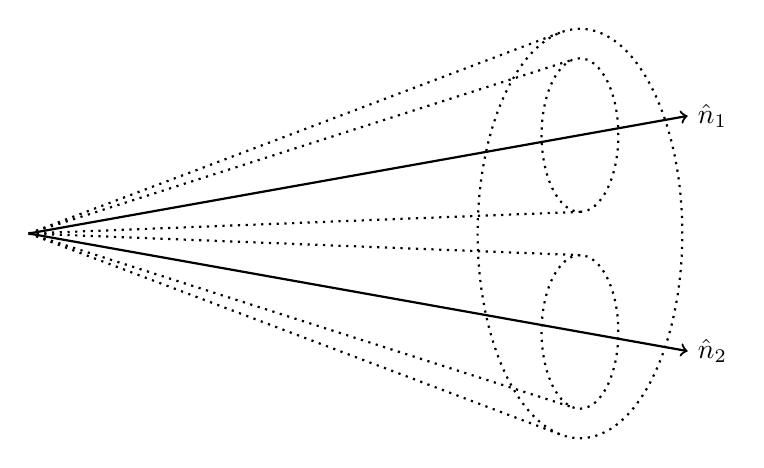
\begin{tikzpicture}
  % Main jet
  \draw[rotate around={270:(0,0)},dotted,thick] (0,7) ellipse (2.6 and 1.3);
  \draw[rotate around={270:(0,0)},dotted,thick] (0,0) -- (69.29:7.21);
  \draw[rotate around={270:(0,0)},dotted,thick] (0,0) -- (110.71:7.21);

  % Subjets
  \draw[rotate around={270:(0,0)},dotted,thick] (1.25,7) ellipse (0.975 and 0.4875);
  \draw[rotate around={270:(0,0)},dotted,thick] (0,0) -- (72.275:7.26);
  \draw[rotate around={270:(0,0)},dotted,thick] (0,0) -- (87.75:7.01);
  \draw[rotate around={270:(0,0)},dotted,thick] (-1.25,7) ellipse (0.975 and 0.4875);
  \draw[rotate around={270:(0,0)},dotted,thick] (0,0) -- (92.25:7.01);
  \draw[rotate around={270:(0,0)},dotted,thick] (0,0) -- (107.725:7.26);

  % Axes
  \draw[->,thick] (0,0) -- (10.12:8.5) node[right] {$\vb{\hat{n}}_1$};
  \draw[->,thick] (0,0) -- (-10.12:8.5) node[right] {$\vb{\hat{n}}_2$};
\end{tikzpicture}

  \caption{
    Illustration of jet substructure for a two-pronged jet with axes $\mathbf{\hat{n}}_1$ and $\mathbf{\hat{n}}_2$.
    The $N$-subjettiness $\tau_N$ is used as a measure of how many subjets are present within a jet.
  }
  \label{fig:jetSubstruct}
\end{figure}

% N-subjettiness ratios
In some cases it is advantageous to consider ratios of $N$-subjettiness.
For example, in this analysis we consider the ratio $\tau_2/\tau_1=\nsubj$, which is a measure of whether or not the jet exhibits the properties we would expect from a jet with 2 subjets versus a single jet with no substructure.
This allows for separating jets originating from boosted vector bosons versus jets that are produced from quarks and gluons, thereby allowing further background suppression.
This analysis uses a modified version of the $N$-subjettiness ratio that reduces the dependency of \nsubj on the jet mass, which is denoted by the designed decorrelated tagger (DDT) $N$-subjettiness \nsubjDDT~\cite{Dolen_2016}.
It is defined by
\begin{equation}
  \nsubjDDT=\nsubj-C\ln\pqty{\frac{\MJ^2}{\ptjet\times(1\unit{GeV})}},
\end{equation}
where $C$ is a coefficient obtained by taking the slope of a fit for the \nsubj profile versus $\ln\pqty{\frac{\MJ^2}{\ptjet\times(1\unit{GeV})}}$ in non-resonant \Wjets background events after applying the full analysis selection cuts.

% N-subjettiness selection
For this analysis, we only consider large-radius jets that satisfy $\nsubjDDT<0.80$.
We also later use \nsubjDDT for event categorization to split the analysis into high and low purity jet categories.

\subsubsection{$b$-tagging}

% CHS approach
While the boosted jets resulting from the \Vhad decay are identified and groomed using algorithms such as the anti-\kt and PUPPI algorithms, the candidate four vector for the $X$ boson is estimated using jet energy scale corrections and charged hadron subtraction (CHS).
The CHS approach is used in order to suppress background contribution from top quark production, which results in the production of jets from $b$ decays.

% b-tagging details
Jets in the region $|\eta|<2.4$ are $b$-tagged if they pass the \texttt{medium} working point of the Combined Secondary Vertex (CSV) or DeepCSV algorithms, as recommended by the $b$-tag and vertexing (BTV) POG.
The \texttt{medium} working point for CSV is 0.8484 in 2016~\cite{bTagging2016}, and for DeepCSV the working points are 0.4941 and 0.4184 for 2017 and 2018, respectively~\cite{bTagging2017,bTagging2018}.
We also apply $b$-tagging scale factors and weights that depend on the jet \pt, $\eta$, and value of the $b$-tagging discriminant as prescribed by the BTV POG~\cite{bTaggingEff,bTaggingSF}.

\subsubsection{$H(b\bar{b})$-tagging}

% The need for bb-tagging
The $V$-tagging methods previously described account for identifying and grooming jets resulting from the $\Vhad$ decay, but additional techniques are applied in this analysis to account for a large-radius \bbbar jet.
Such a jet signifies the decay \Htobbbar in the final state and hence a \WH resonance, which allows for discriminating against background with light jet flavors.
For this reason, we use a $b$-tagging discriminator to identify Higgs boson jet candidates that uses information from displaced tracks and secondary vertices~\cite{CMS-PAS-BTV-15-002}.
We also apply a cut on the M2 operating point of the ``\DoubleB tagger'' to categorize events, for which the threshold is 0.8 for Run 2 according to references~\cite{bTagging2016,bTagging2017,bTagging2018}.

% Scale factors
Additionally, we apply scale data/MC efficiency scale factors to our signal sample normalizations as recommended by the BTV POG, while the scale factors for the background are estimated from the data in the control regions.
We use two sets of scale factors that depend on \ptjet.
One is for \Htobbbar jets resulting from the \WprtoWHtolnubbbar signal model, and the other is for mistagging $W$ bosons resulting from $t\bar{t}$ events, which are applied to the \GBulktoWWtolnuqqbarpr and \WprtoWZtolnuqqbar signal models.
These scale factors are applied from method 1a from reference~\cite{bTaggingEff}.
First we measure the MC \bbbar-tagging efficiencies $\epsilon$, then apply the event weights for the \bbbar-tagged category as
\begin{equation}
  w^{\bbbar}(\pt)=\frac{\mathrm{SF}(\pt)\epsilon(\pt)}{\epsilon(\pt)}=\mathrm{SF}(\pt),
\end{equation}
where $\mathrm{SF}$ denotes the scale factors.
For the \bbbar-untagged category, we instead use
\begin{equation}
  w^{\mathrm{no}\bbbar}(\pt)=\frac{1-\mathrm{SF}(\pt)\epsilon(\pt)}{1-\epsilon(\pt)}.
\end{equation}

\subsection{Missing Transverse Energy}

% MET
For this analysis, we use type-I corrected particle flow MET (PFMET) to account for the energy of the neutrino from the \Wlep decay, where PFMET is defined as the magnitude of the negative vector sum of all transverse energies from particle flow objects~\cite{PFMET}.
The correction is a propagation of the jet energy corrections (JEC) to MET, which is given by
\begin{equation}
  \EtmissTI=\vqty{-\sum_\mathrm{jet}\mathbf{p}_\mathrm{T,jet}^\mathrm{JEC}-\sum_{i\in\mathrm{uncl.}}\mathbf{p}_{\mathrm{T},i}},
\end{equation}
where the first sum is over clustered jets and the second sum is over unclustered particles.

\subsection{Leptonic $W$ and \WV reconstruction}

% Leptonic reconstruction
To reconstruct the leptonically decaying $W$ candidate \Wlep, we select the highest \pt lepton in the event and combine it with the \EtmissTI resulting from the neutrino.
We also apply a $W$ mass constraint to estimate the $z$-component of the missing energy.
The resulting \Wlep is then combined with the large-radius \Vhad jet to form a diboson candidate, with mass denoted by \MVV.

\subsection{VBF Forward Jets}
\label{subsec:VBFjets}

% VBF signature
The defining signature of the \VBF production process is the presence of two boosted jets in the forward and backward regions of the detector, along with the decay products in the central region of the detector resulting from the \Wlep and \Vhad resonances.
The analysis therefore requires additional kinematic constraints in order to categorize \VBF-produced events, which take into account properties of the forward-facing \VBF jets such as their combined mass and separation in $\eta$.

% VBF jet selection
We select candidate \VBF jets from the two highest \pt standard AK4 jets as defined in subsection~\ref{subsec:jetSelect}.
This requires that the \VBF jets pass $\pt>30\unit{GeV}$, and that they do not overlap with the selected lepton and large-radius jet.
We then apply selection cuts to the two candidate \VBF jets based on their separation in pseudorapidity \DetaVBF and \VBF dijet mass \mjjVBF.

% VBF Deta selection cut
For the cut on \DetaVBF, we exploit the fact that the \VBF jets are expected to be found in the high $|\eta|$ regions of the detector near the endcaps and be roughly anti-parallel to each other.
Figure~\ref{fig:detaSB_VBF} (left) shows the relative shape differences in \DetaVBF between the \VBF\RadtoWW signal MC sample and the background MC samples used in this analysis.
To retain a signal efficiency of 40-50\%, we choose a cut of $\DetaVBF>4$.

\begin{figure}[htbp]
  \centering
  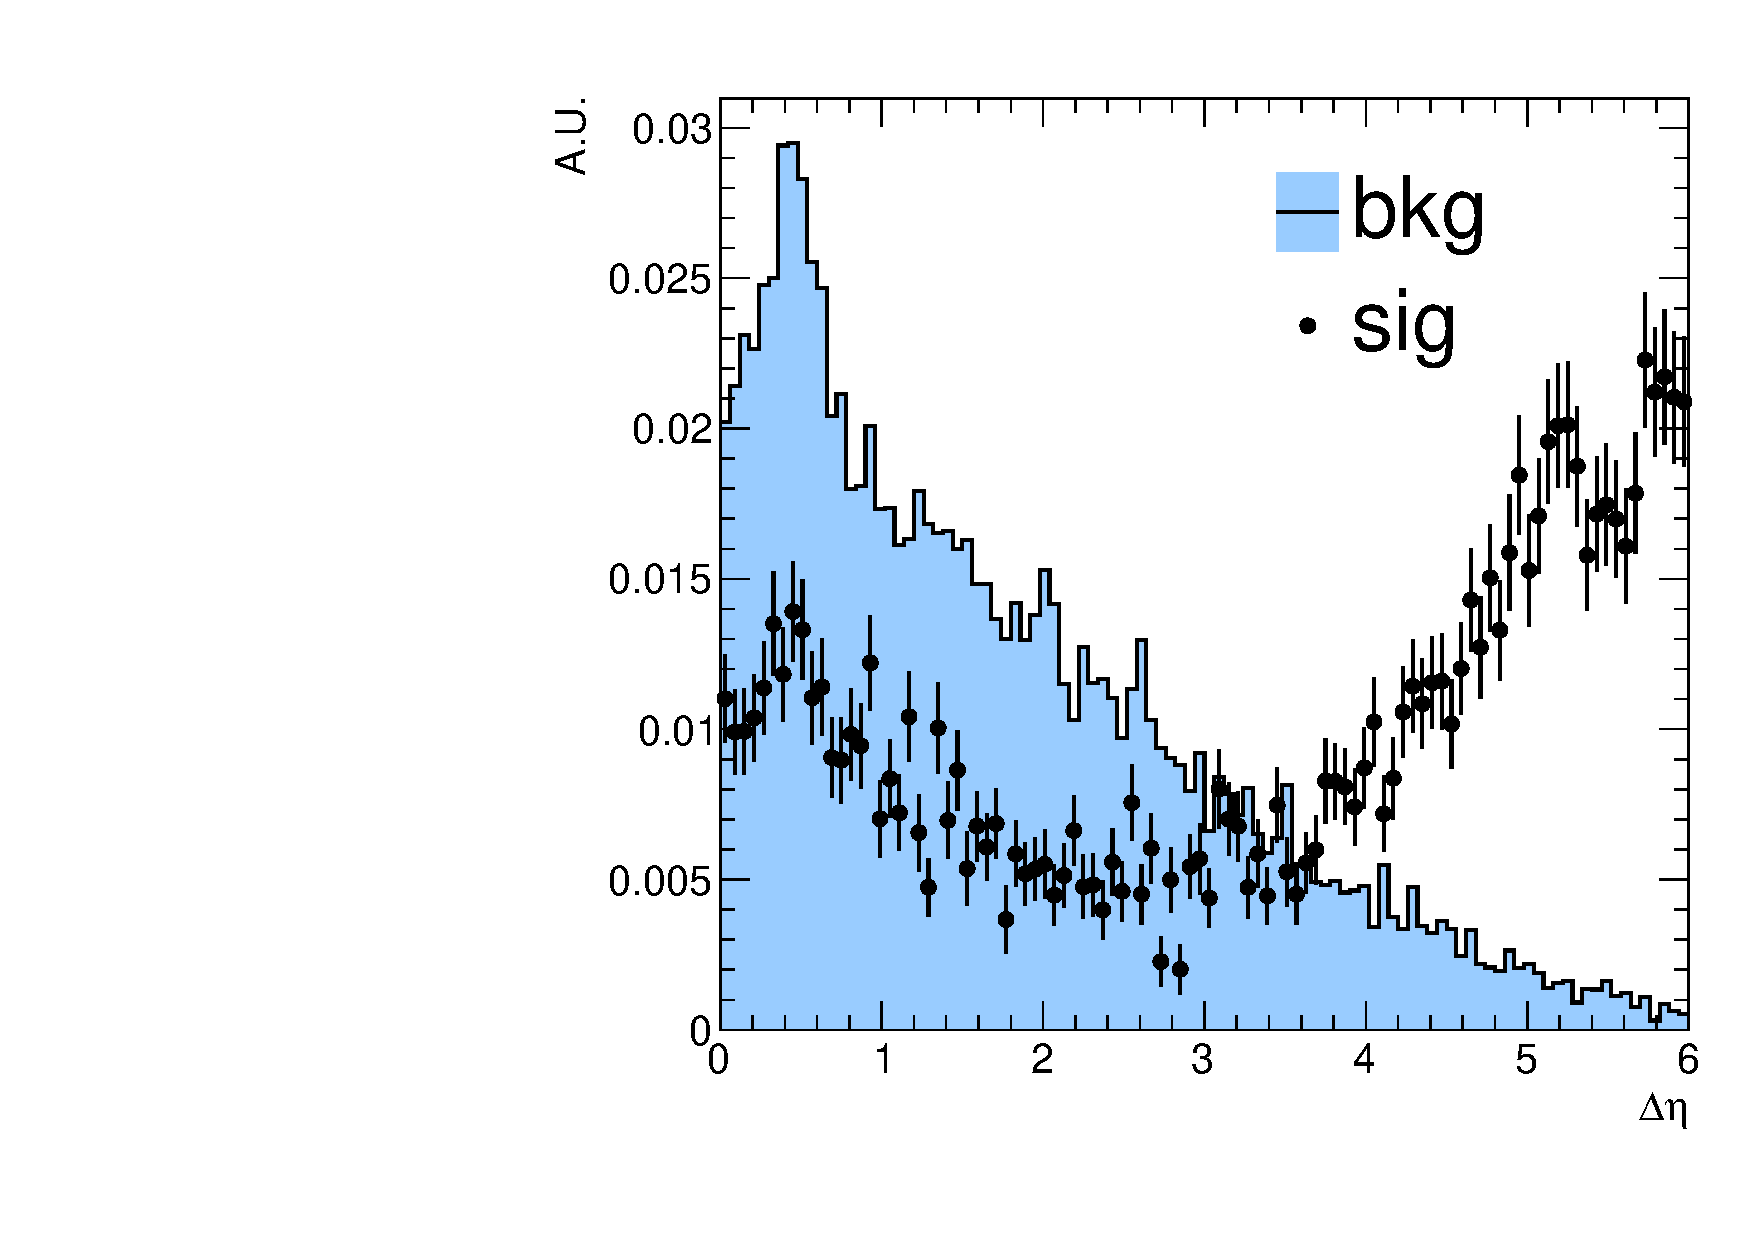
\includegraphics[width=0.45\textwidth]{fig/eventSelection/detaSB.pdf}
  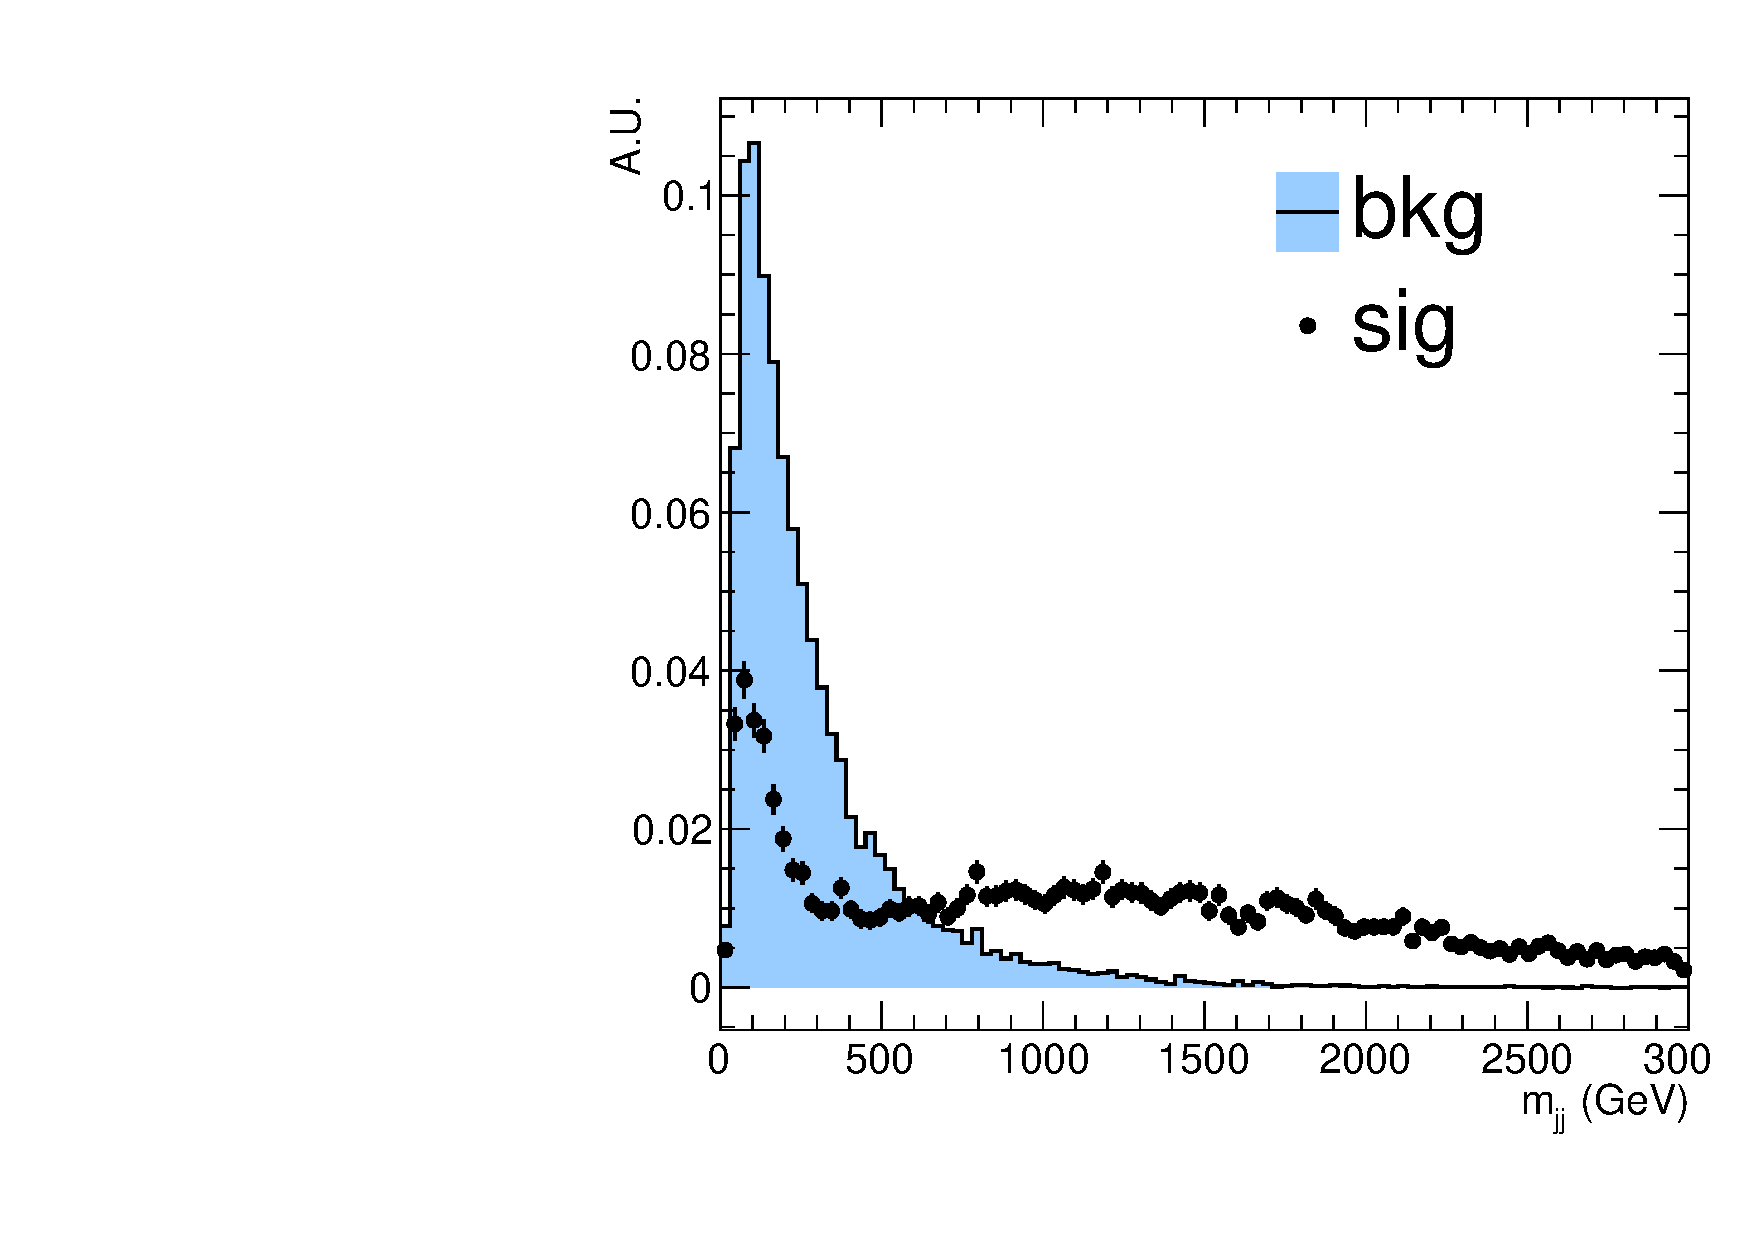
\includegraphics[width=0.45\textwidth]{fig/eventSelection/mjjSB.pdf}
  \caption{
    Shape comparison of a \VBF\RadtoWW signal sample and background MC samples, normalized to unity, for \DetaVBF (left) and \mjjVBF (right).
    The shape discrepancy between the \VBF signal and background distributions in \DetaVBF and \mjjVBF allows for distinguishing signal from background.
  }
  \label{fig:detaSB_VBF}
\end{figure}

% VBF dijet mass selection cut
The other kinematic cut applied to the \VBF candidate jets is on the invariant mass of the sum of the \VBF jet four vectors, \mjjVBF.
For this cut, we consider the Punzi significance obtained for a \VBF signal sample as a function of the thresholds of the cuts for \DetaVBF and \mjjVBF.
The Punzi significance is defined by $\epsilon/(1.5+\sqrt{B})$, where $\epsilon$ is the number of signal events obtained by the cuts assuming an integrated luminosity of $\mathcal{L}_\mathrm{int}=1\unit{pb^{-1}}$ and a cross section of $\sigma=1\unit{pb}$, while the number of background events $B$ is weighted with the total luminosity~\cite{Punzi:2003bu}.
Figure~\ref{fig:detaMjjSB_VBF} shows the Punzi significance for the \VBF\RadtoWW signal sample in the plane spanned by the thresholds for the \DetaVBF and \mjjVBF cuts.
We again require that the selection cut on \mjjVBF retains 40-50\% signal efficiency, as we did for \DetaVBF.
This leads to a cut of $\mjjVBF>500\unit{GeV}$.

\begin{figure}[htbp]
  \centering
  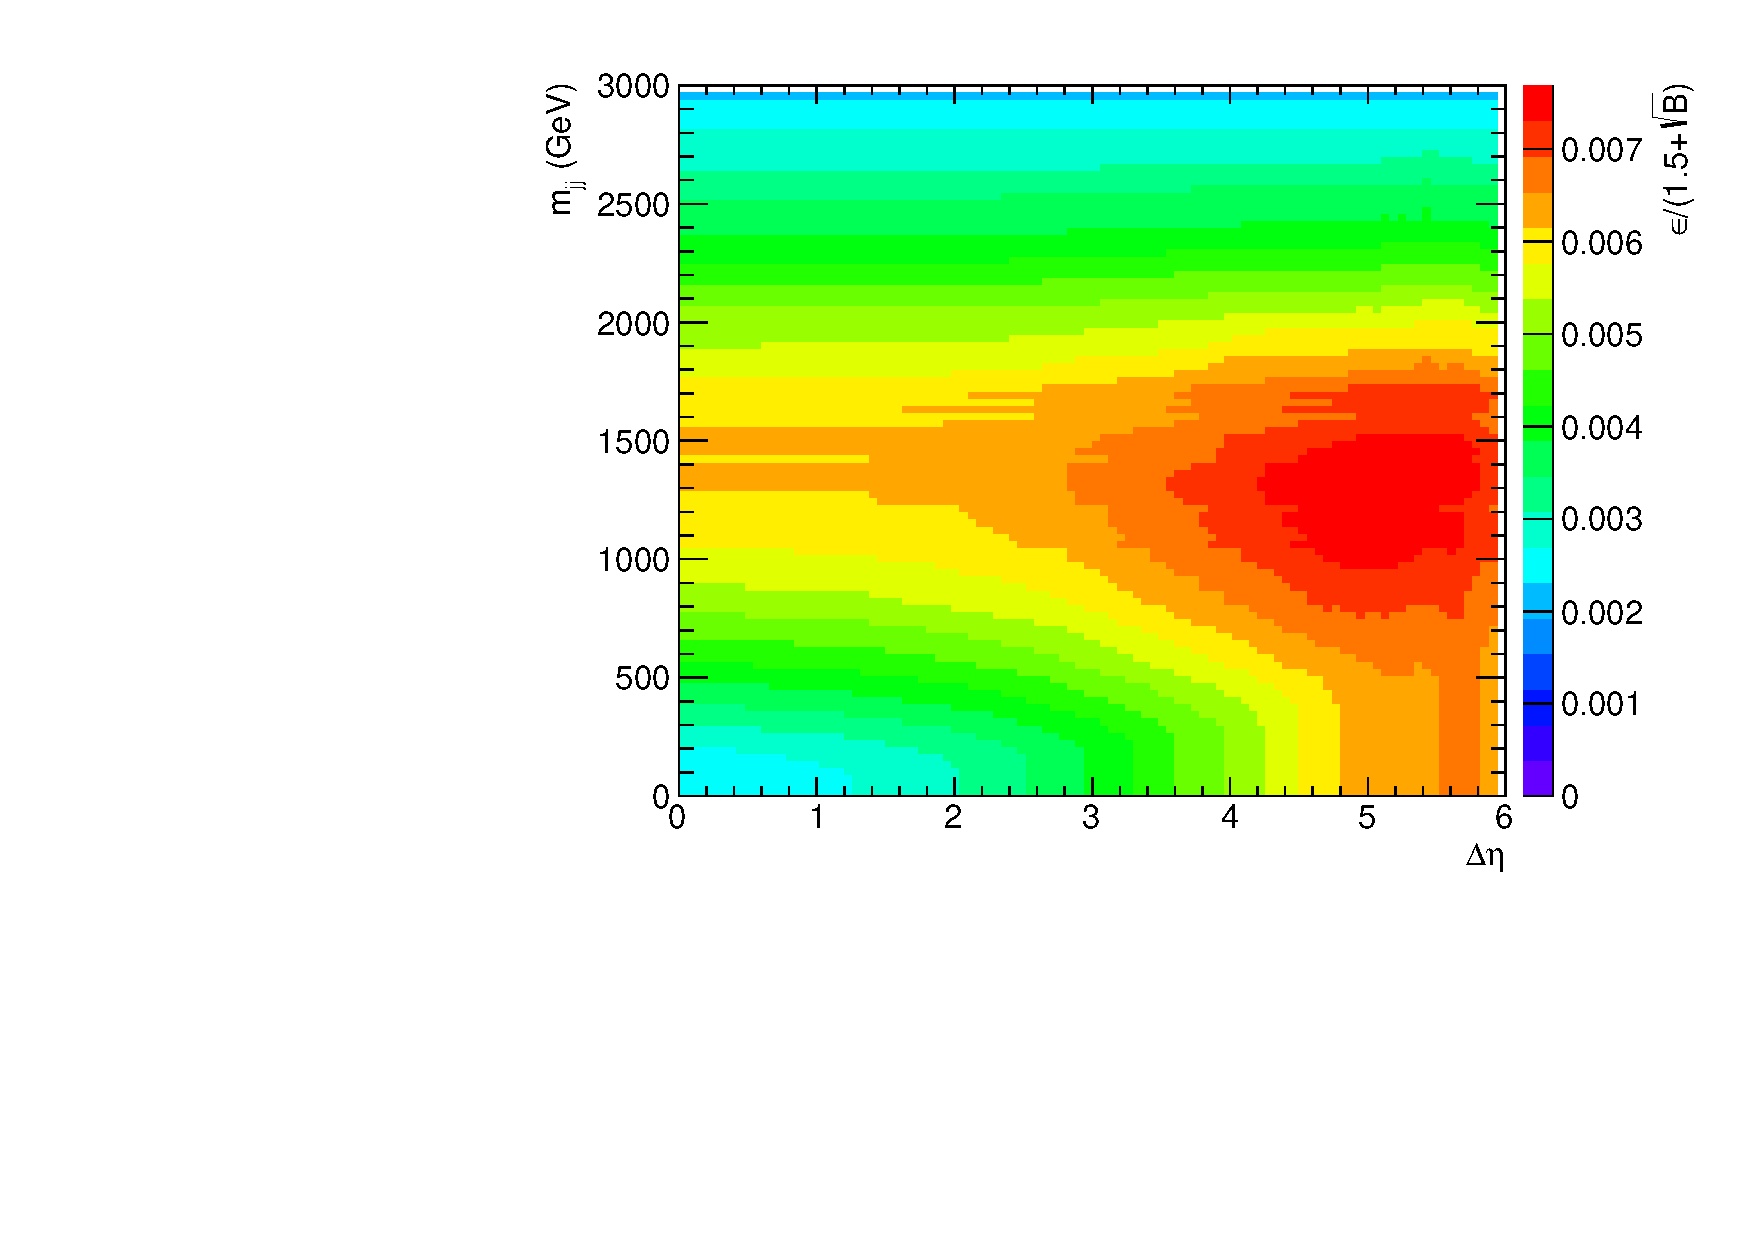
\includegraphics[width=0.5\textwidth]{fig/eventSelection/detaMjjSB.pdf}
  \caption{
    Two-dimensional Punzi significance of the \VBF\RadtoWW signal in the plane of the two thresholds of the cuts on \DetaVBF and \mjjVBF.
  }
  \label{fig:detaMjjSB_VBF}
\end{figure}

\subsection{Spin Polarization and Boson Rapidities}
\label{subsec:spinPol}

% Spin polarization from VBF production
The \VBF production process has another distinctive feature in which some kinematic variables are sensitive to the spin of the $X$ resonance, thereby providing the ability to distinguish between signal models.
This effect can be seen in the distributions for the separation in rapidity between the \Vhad and \Wlep diboson system, which we denote by \Dy.
Figure~\ref{fig:DyComp} shows the shape discrepancies between the MC signals and backgrounds in \Dy, separated by non-\VBF (left) and \VBF-produced signals.

\begin{figure}[htbp]
  \centering
  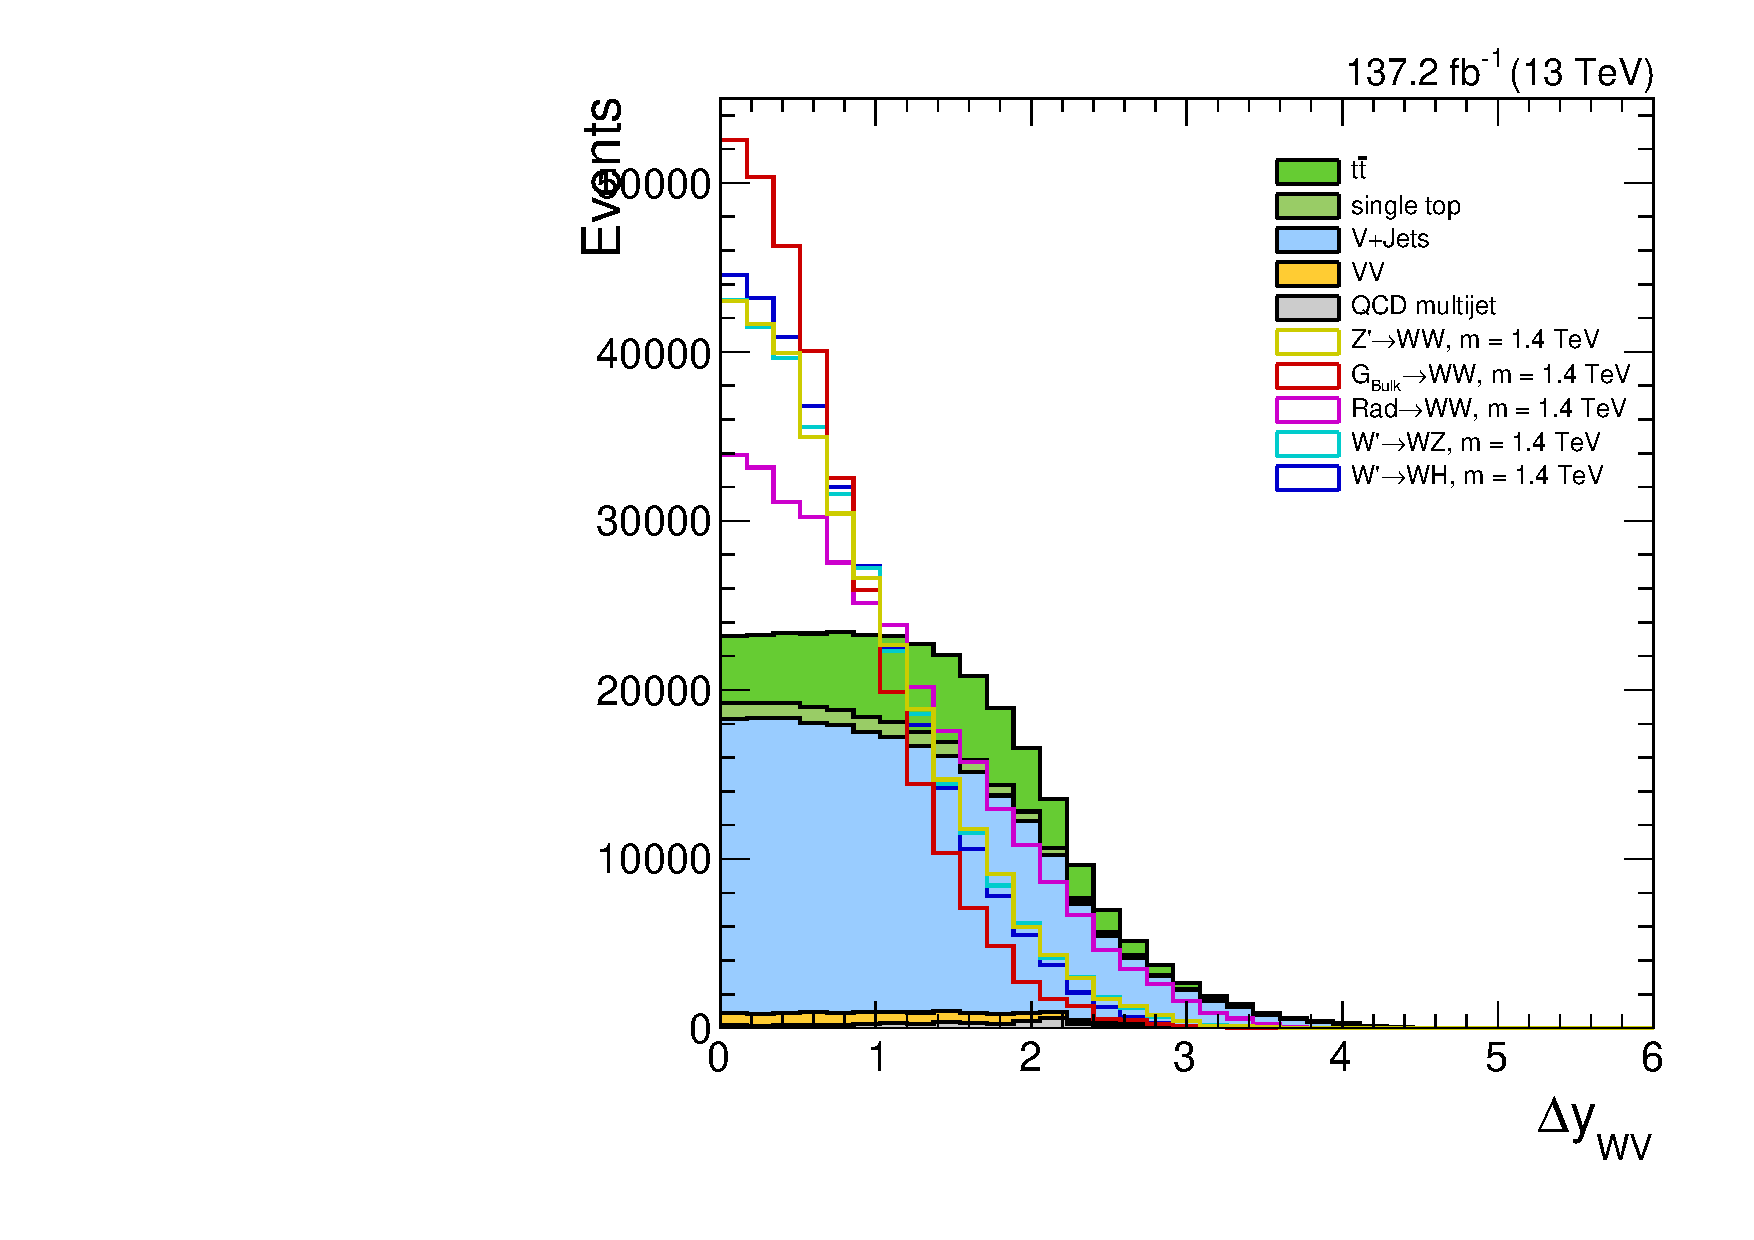
\includegraphics[width=0.45\textwidth]{fig/eventSelection/SR_b1_allL_allP_allC_inc_lo_Run2_Dy.pdf}
  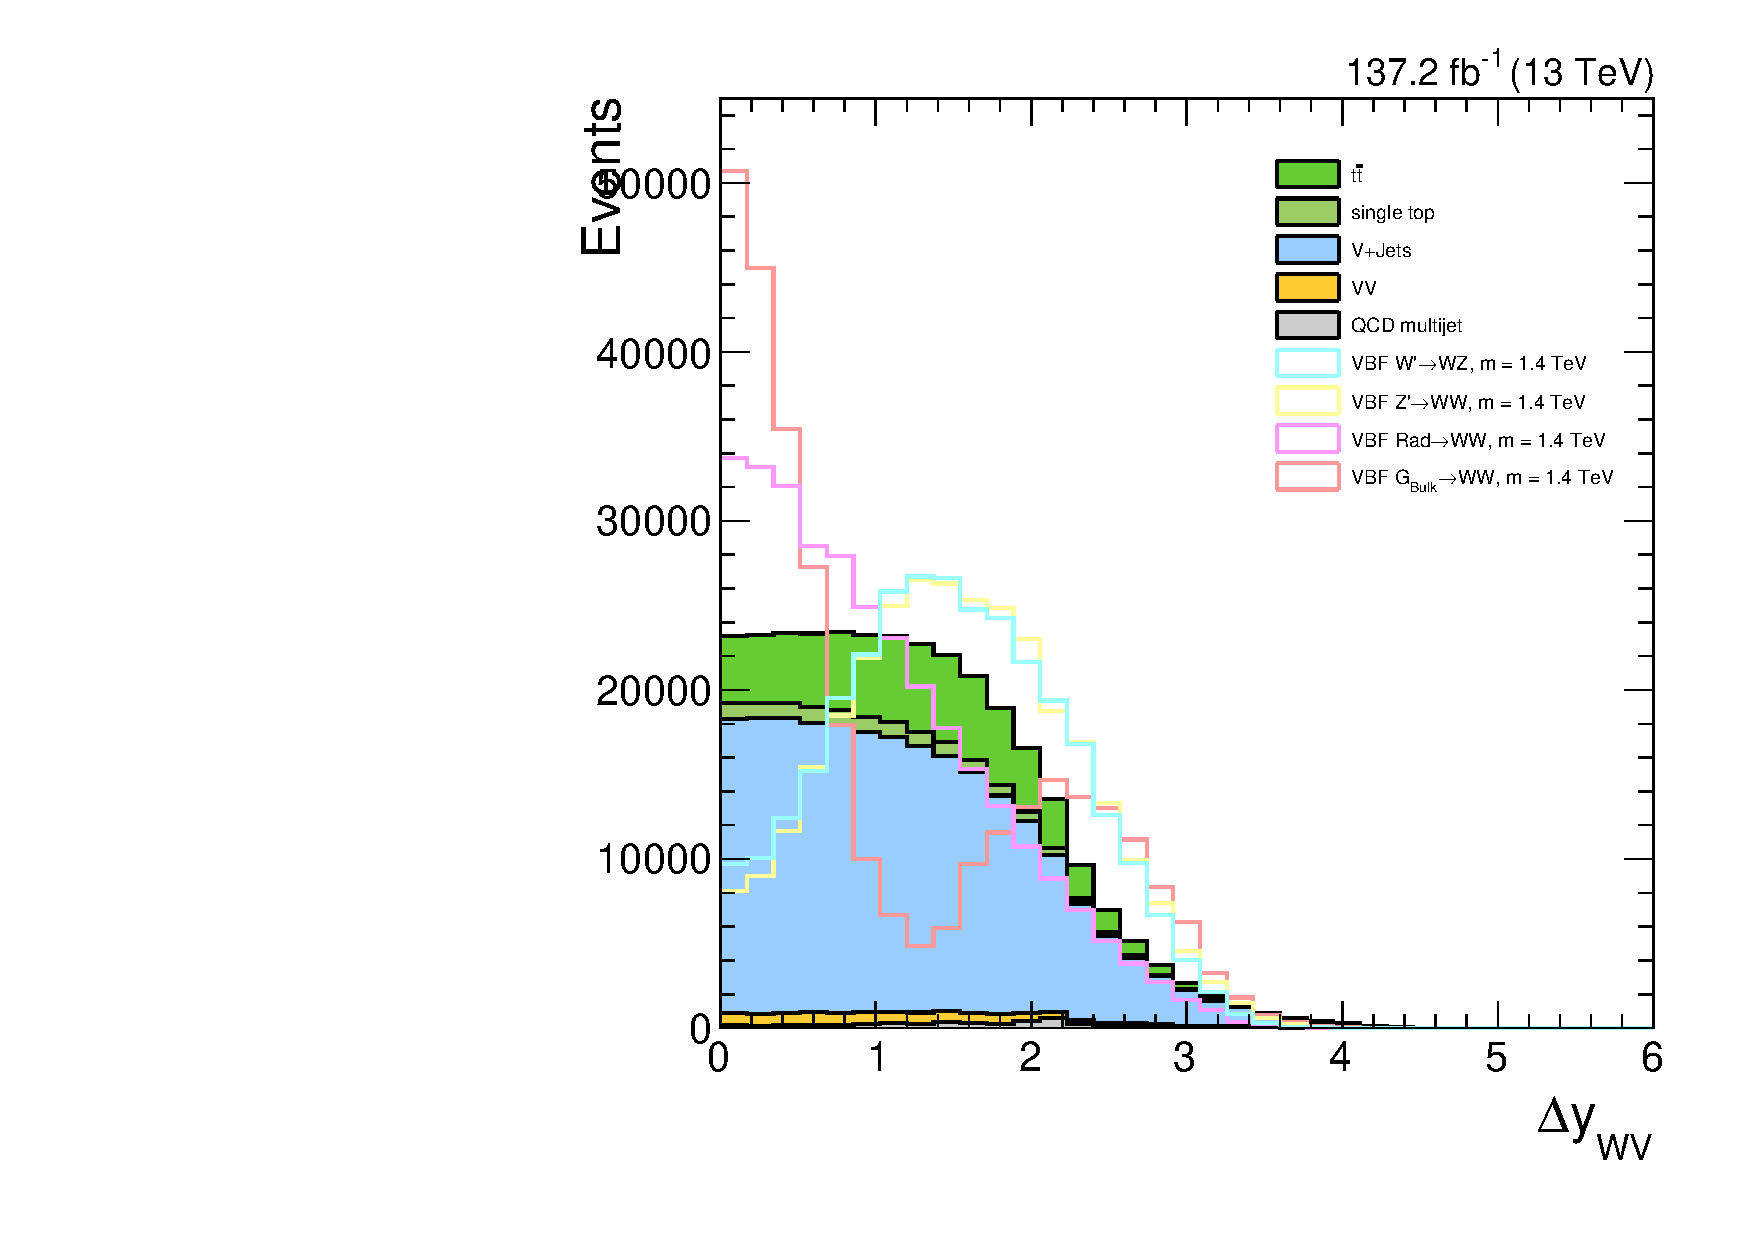
\includegraphics[width=0.45\textwidth]{fig/eventSelection/SR_b1_allL_allP_allC_vbf_lo_Run2_Dy.pdf}
  \caption{
    Shape comparison of the angular separation \Dy between the two reconstructed bosons for simulated background and signals, in the signal region.
    Backgrounds distributions are stacked and normalized to the expected luminosity for the full Run-2, while signal distributions are overlaid, all arbitrarily normalized to the same integral as the sum of backgrounds.
    Non-\VBF (left) and \VBF (right) signals are shown separately.
    The shape differences between signals is most apparent in the case of \VBF production, allowing for distinguishing between spin-0, spin-1, and spin-2 signals.
    This defines a new layer of categorization for the analysis.
  }
  \label{fig:DyComp}
\end{figure}

% Non-VBF signals
The signals produced via \ggF or \DY have minor shape differences between each other, and their distributions are consistently narrower and more concentrated in the low \Dy region compared to the background MC samples.
This on its own suggests that categorizing the search based on \Dy would increase the search sensitivity.

% VBF signals
For the \VBF-produced signals, the shape differences between signals are much more apparent.
The spin-1 \VBF\WprtoWZ and \ZprtoWW signals both peak around $\Dy=1.4$ rather than plateauing like the background from $\Dy=0$ to 0.8.
Meanwhile, the spin-2 \VBF\GBulktoWW signal has two peaks, with a large and narrow peak occurring at $\Dy=0$, followed by a smaller peak around $\Dy=2.0$.
Finally, the \VBF\RadtoWW signal exhibits no difference in its \Dy distribution compared to the \ggF\RadtoWW signal since it is a spin-0 resonance, but it still differs from the other \VBF signals since it only has a peak at $\Dy=0$.

% Statistical power of Dy categories
The shape differences between the \VBF signals allow for not only enhancing the search sensitivity by using categories based on \Dy, but by also allowing for distinguishing between spin-0 (\RadtoWW), spin-1 (\ZprtoWW, \WprtoWZ, \WprtoWH), or spin-2 (\GBulktoWW) \VBF signal models.
For this reason, we use two categories based on rapidity: a low-\Dy category defined by the condition $\Dy<1.0$, and a high-\Dy category defined by $\Dy\geq1.0$.
Originally a 3-category scheme was considered for the analysis, but it was found that this did not leave sufficient background MC statistics in all three categories in order to build robust 2D background templates.

\subsection{Final Event Selection and Categorization}
\label{subsec:eventSelect}

% Event selection and categorization
For this analysis, we made a final event selection in order to select events that exhibit the expected behavior of the final state described in subsection~\ref{subsec:expEvent} and optimize the search potential for a semileptonically decaying heavy $X$ resonance produced via \ggF, \DY, or \VBF.
We then divide the analysis into disjoint categories in order to enhance the search sensitivity.

\subsubsection{Final Event Selection}

% Final event selection
The final event selection used in the analysis is defined by the following:
\begin{enumerate}
  \item Exactly one charged lepton as defined in subsections~\ref{subsec:muonSelect} and \ref{subsec:elecSelect}.
  \item Lepton veto: no additional loose electron ($\pt>35\unit{GeV}$) or muon ($\pt>20\unit{GeV}$) in the event.
  \item Type-I corrected missing transverse energy \EtmissTI: events are required to have $\Etmiss>80\unit{GeV}$ for the electron channel and $\Etmiss>40\unit{GeV}$ for the muon channel to suppress contributions from QCD multijet backgrounds.
  \item Leptonic $W$ \pt: the \pt of the reconstructed \Wlep must satisfy $\pt>200\unit{GeV}$ in order to select a boosted $W$ topology.
  \item Hadronic \VorH \pt: the \pt of the reconstructed \Vhad must satisfy $\pt>200\unit{GeV}$ in order to select a boosted \VorH topology.
  \item $b$-tag veto: the event is required to have no $b$-tagged standard jets.
  \item \ZH veto: to ensure that the selection is disjoint from the $X\to\ZH\to\ell\ell\bbbar$ search~\cite{CMS_AN2019_107}, which uses a different electron and muon ID, we explicitly veto events where a \ZH candidate is selected with their criteria.
  \item Search region: the search region is defined as $0.6<\MVV<5.0\unit{TeV}$ and $20<\MJ<210\unit{GeV}$.
\end{enumerate}

\subsubsection{Final Event Categories}
\label{subsec:eventCat}

% Final event categories
After considering the final event selection, we split the analysis into 24 disjoint event categories.
The categories are based on four successive criteria based on the lepton channel, large-radius jet purity, \VBF/non-\VBF categories, and \Dy categories.

% Lepton channel
First, we split the event sample based on the lepton flavor of the reconstructed \Wlep candidate, defining two channels:
\begin{itemize}
  \item {\bfseries Electron channel ($e$)}
  \item {\bfseries Muon channel ($\mu$)}
\end{itemize}

% Jet purity
Second, we exploit the fact that the jets originating from \VorH decays exhibit a two-pronged structure.
The analysis is split based on $V$-jet tagging via cuts on the value of the mass-decorrelated $N$-subjettiness ratio \nsubjDDT as described in subsection~\ref{subsec:jetSelect}.
This defines the following two categories:
\begin{itemize}
  \item {\bfseries High Purity (HP):} $\nsubjDDT<0.50$
  \item {\bfseries Low Purity (LP):} $0.50<\nsubjDDT<0.80$
\end{itemize}

% VBF/non-VBF categories
Third, to enhance the sensitivity of resonances decaying to \WHtolnubbbar, and to separate events consistent with \VBF production, we split the sample three-way based on the value of the \DoubleB tagger and the presence of \VBF-compatible jet candidates described in subsection~\ref{subsec:VBFjets}:
\begin{itemize}
  \item {\bfseries \VBF-tagged (vbf):} Two candidate \VBF jets, $\DetaVBF>4$, $\mjjVBF>500\unit{GeV}$
  \item {\bfseries \bbbar-tagged (bb):} $\DoubleB>0.8$, no \VBF tag
  \item {\bfseries \bbbar-untagged (nobb):} $\DoubleB<0.8$, no \VBF tag
\end{itemize}

% Dy categories
Fourth, to further discriminate all signals against background and distinguish between \VBF-produced signals of different spins, we split the sample using the diboson rapidity separation \Dy between the \Wlep and \Vhad as discussed in subsection~\ref{subsec:spinPol}:
\begin{itemize}
  \item {\bfseries Low \Dy (LDy):} $\Dy<1.0$
  \item {\bfseries High \Dy (HDy):} $\Dy\geq1.0$
\end{itemize}

This selection defines $2\times2\times3\times2=24$ search categories that are referred to with labels such as e-HP-bb-LDy, $\mu$-LP-vbf-HDy, etc.
